\documentclass[class=../report, crop=false]{standalone}
\usepackage[subpreambles=true]{standalone}
\usepackage{graphicx}

\begin{document}

\section{Functional Decomposition}

We applied \gls{funcdecomp} to reduce the complexity of designing a locomotive.
%We reduced the complexity of designing a locomotive by applying \gls{funcdecomp}. %Ghetto space hack for glsgenentry screws up the period
Using our design objectives as guidelines, we identified the functions that the locomotive must complete.
We dissected the problem into the \gls{toplevel} shown in Figure \ref{fig:toplevel}.

\begin{figure}[h]
	\centering
	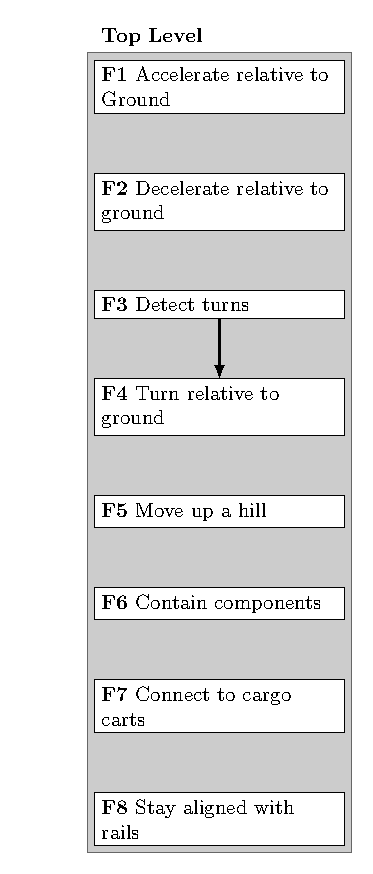
\includegraphics{../../bin/toplevel.pdf}
	\caption{Top-Level Functions}
	\label{fig:toplevel}
\end{figure}

\clearpage

We generated \gls{conceptfrags} for each of the top level functions, prioritizing quantity and creativity.
We ignored regulations during ideation to stimulate creativity.
Some concept fragments had subfunctions that needed to be addressed for them to be incorporated.
We used a function structure diagram to organize the concept fragments; an example of the function decomposition for the function Turn Relative to Ground is displayed below in Figure \ref{fig:turn-relative-to-ground}.

\begin{figure}[h!]
	\centering
	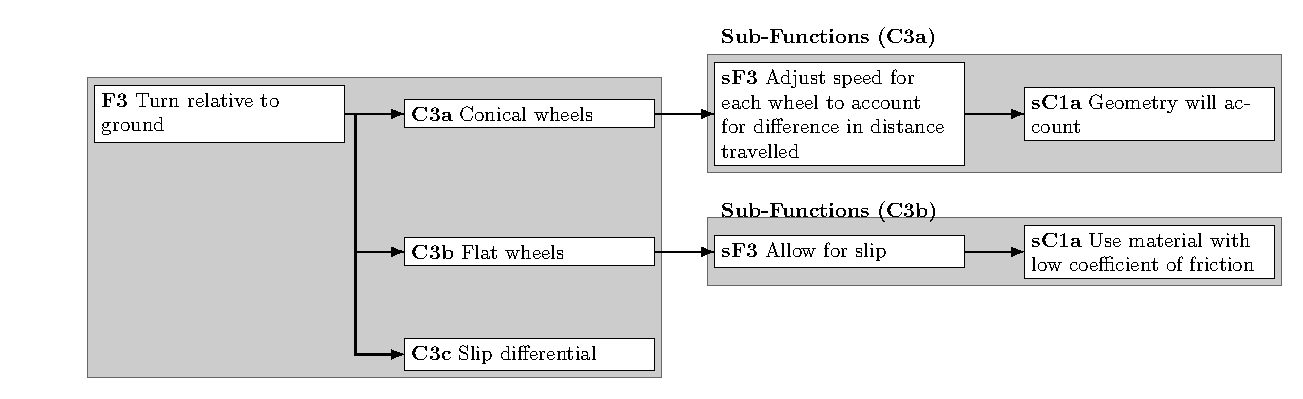
\includegraphics[width=\textwidth]{../../bin/turn_relative_to_ground.pdf}
	\caption{Functional Decomposition, Turn Relative to Ground}
	\label{fig:turn-relative-to-ground}
\end{figure}

The clear separation between different functions allowed us to quickly generate ideas for each function.
The full function structure diagram is found in Appendix \ref{app:funcdecomp}: \nameref{app:funcdecomp}.

\end{document}
